\section{Computational Companion}
\label{sec:ch3-computational}

Numerical and symbolic tools are most valuable when they expose geometry rather than replace reasoning. The companion programs reproduce the field plots and verify representative identities using finite differences.

\subsection{Python workflow}
The file \texttt{examples/python/ch03/vector\_calculus\_companion.py} generates four publication-ready figures and reports numerical checks for divergence, curl, flux, and circulation.

\begin{lstlisting}[language=Python,caption={Core numerical field operations used in the Chapter 3 companion.}]
def divergence(Fx, Fy, dx, dy):
    dFx_dx = np.gradient(Fx, dx, axis=1)
    dFy_dy = np.gradient(Fy, dy, axis=0)
    return dFx_dx + dFy_dy

def scalar_curl(Fx, Fy, dx, dy):
    dFy_dx = np.gradient(Fy, dx, axis=1)
    dFx_dy = np.gradient(Fx, dy, axis=0)
    return dFy_dx - dFx_dy
\end{lstlisting}

\begin{bookfigure}{Computational field gallery: a rotational field, its curl, flux through a circle, and diffusion smoothing.}{fig:ch3-computational-gallery}
\begin{minipage}{\textwidth}
\centering
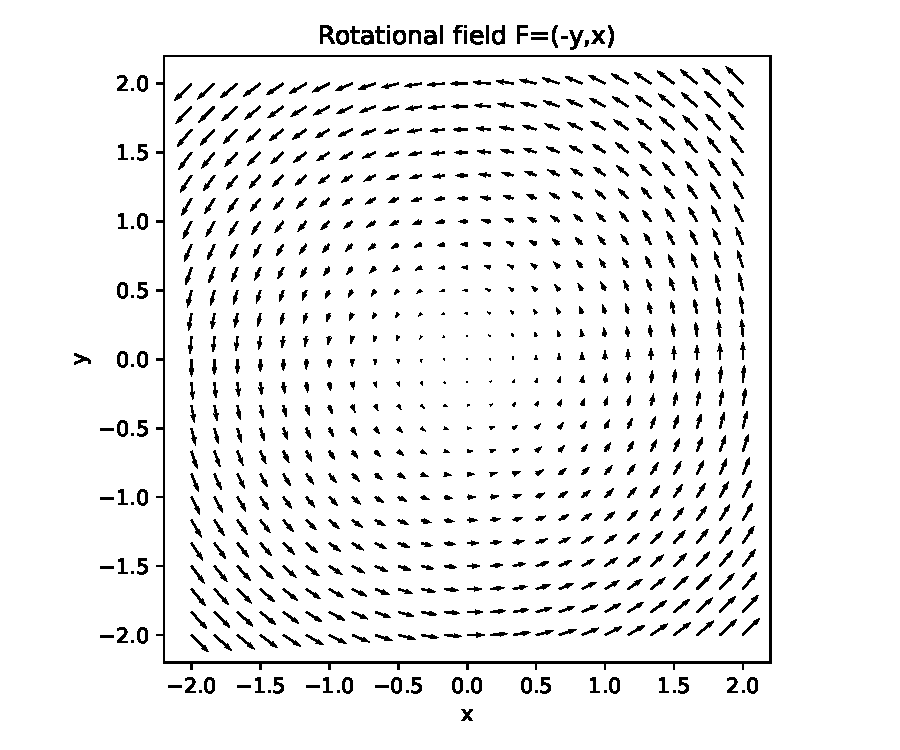
\includegraphics[width=0.47\textwidth]{generated/ch03/rotational_field.pdf}\hfill
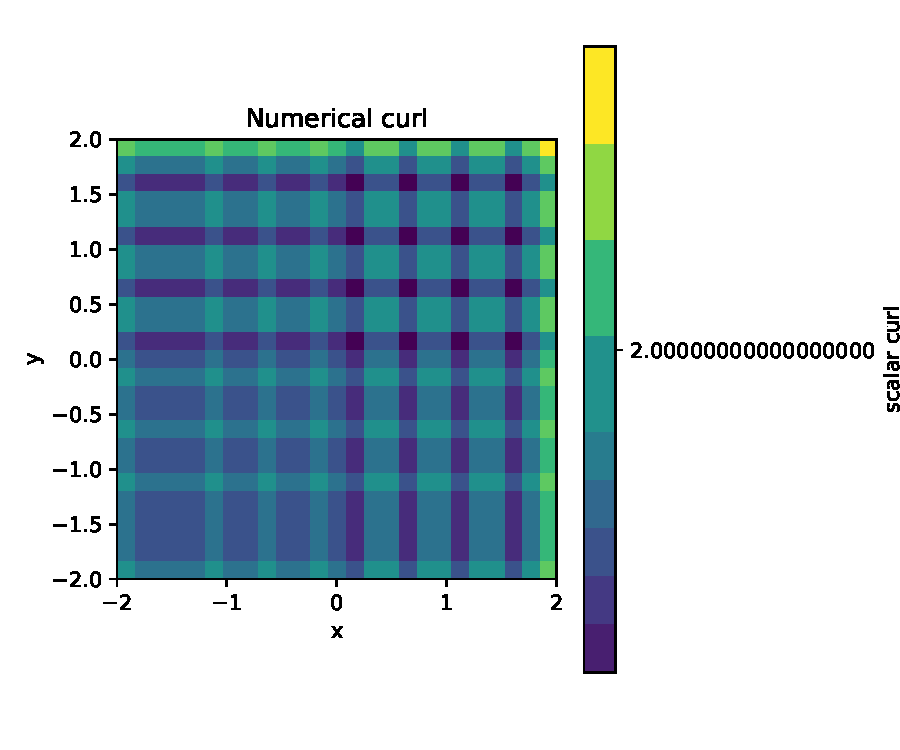
\includegraphics[width=0.47\textwidth]{generated/ch03/curl_map.pdf}\par\medskip
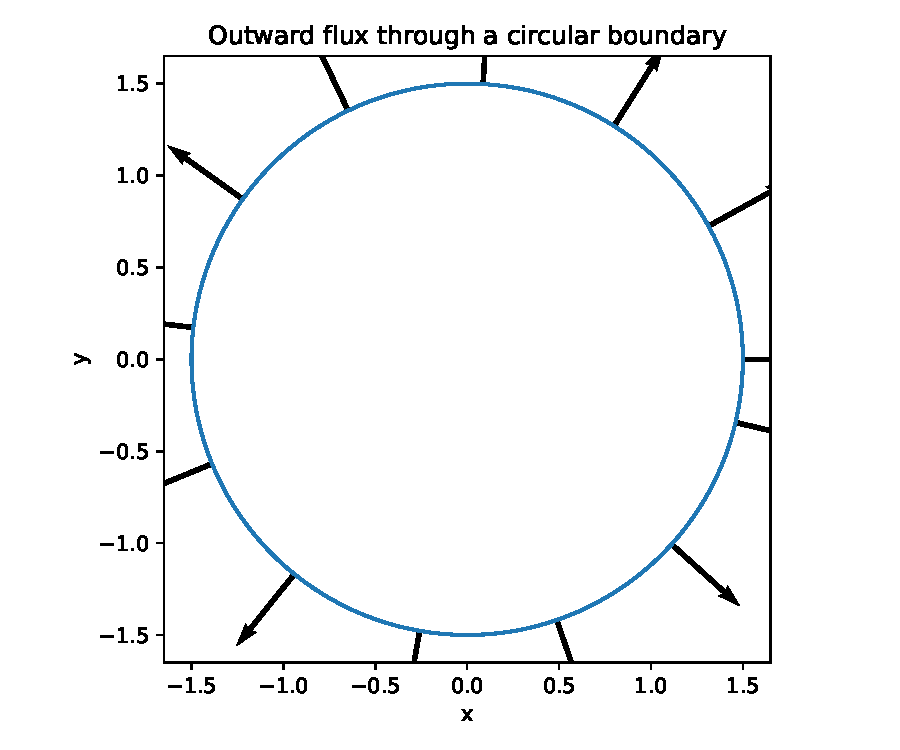
\includegraphics[width=0.47\textwidth]{generated/ch03/flux_circle.pdf}\hfill
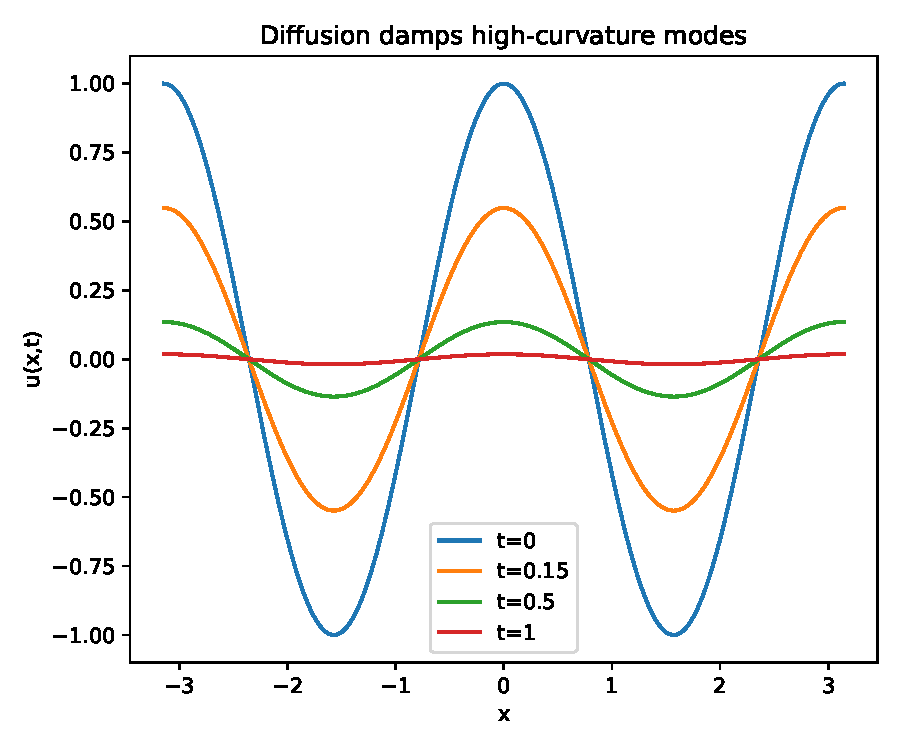
\includegraphics[width=0.47\textwidth]{generated/ch03/diffusion_modes.pdf}
\end{minipage}
\end{bookfigure}

\subsection{Wolfram Language workflow}
The matching file \texttt{examples/wolfram/ch03/vector\_calculus\_companion.wl} demonstrates symbolic evaluation of $\nabla\cdot\mathbf F$, $\nabla\times\mathbf F$, and the three integral theorems. Keeping both implementations makes the mathematical intent independent of one software ecosystem.

\begin{warningbox}
A visually smooth field plot is not evidence that a derivative or integral has been computed correctly. Always test convergence under grid refinement and compare against an analytic case whose answer is known.
\end{warningbox}
